% Options for packages loaded elsewhere
\PassOptionsToPackage{unicode}{hyperref}
\PassOptionsToPackage{hyphens}{url}
\PassOptionsToPackage{dvipsnames,svgnames,x11names}{xcolor}
%
\documentclass[
  letterpaper,
  DIV=11,
  numbers=noendperiod]{scrartcl}

\usepackage{amsmath,amssymb}
\usepackage{iftex}
\ifPDFTeX
  \usepackage[T1]{fontenc}
  \usepackage[utf8]{inputenc}
  \usepackage{textcomp} % provide euro and other symbols
\else % if luatex or xetex
  \usepackage{unicode-math}
  \defaultfontfeatures{Scale=MatchLowercase}
  \defaultfontfeatures[\rmfamily]{Ligatures=TeX,Scale=1}
\fi
\usepackage{lmodern}
\ifPDFTeX\else  
    % xetex/luatex font selection
\fi
% Use upquote if available, for straight quotes in verbatim environments
\IfFileExists{upquote.sty}{\usepackage{upquote}}{}
\IfFileExists{microtype.sty}{% use microtype if available
  \usepackage[]{microtype}
  \UseMicrotypeSet[protrusion]{basicmath} % disable protrusion for tt fonts
}{}
\makeatletter
\@ifundefined{KOMAClassName}{% if non-KOMA class
  \IfFileExists{parskip.sty}{%
    \usepackage{parskip}
  }{% else
    \setlength{\parindent}{0pt}
    \setlength{\parskip}{6pt plus 2pt minus 1pt}}
}{% if KOMA class
  \KOMAoptions{parskip=half}}
\makeatother
\usepackage{xcolor}
\setlength{\emergencystretch}{3em} % prevent overfull lines
\setcounter{secnumdepth}{-\maxdimen} % remove section numbering
% Make \paragraph and \subparagraph free-standing
\ifx\paragraph\undefined\else
  \let\oldparagraph\paragraph
  \renewcommand{\paragraph}[1]{\oldparagraph{#1}\mbox{}}
\fi
\ifx\subparagraph\undefined\else
  \let\oldsubparagraph\subparagraph
  \renewcommand{\subparagraph}[1]{\oldsubparagraph{#1}\mbox{}}
\fi


\providecommand{\tightlist}{%
  \setlength{\itemsep}{0pt}\setlength{\parskip}{0pt}}\usepackage{longtable,booktabs,array}
\usepackage{calc} % for calculating minipage widths
% Correct order of tables after \paragraph or \subparagraph
\usepackage{etoolbox}
\makeatletter
\patchcmd\longtable{\par}{\if@noskipsec\mbox{}\fi\par}{}{}
\makeatother
% Allow footnotes in longtable head/foot
\IfFileExists{footnotehyper.sty}{\usepackage{footnotehyper}}{\usepackage{footnote}}
\makesavenoteenv{longtable}
\usepackage{graphicx}
\makeatletter
\def\maxwidth{\ifdim\Gin@nat@width>\linewidth\linewidth\else\Gin@nat@width\fi}
\def\maxheight{\ifdim\Gin@nat@height>\textheight\textheight\else\Gin@nat@height\fi}
\makeatother
% Scale images if necessary, so that they will not overflow the page
% margins by default, and it is still possible to overwrite the defaults
% using explicit options in \includegraphics[width, height, ...]{}
\setkeys{Gin}{width=\maxwidth,height=\maxheight,keepaspectratio}
% Set default figure placement to htbp
\makeatletter
\def\fps@figure{htbp}
\makeatother
\newlength{\cslhangindent}
\setlength{\cslhangindent}{1.5em}
\newlength{\csllabelwidth}
\setlength{\csllabelwidth}{3em}
\newlength{\cslentryspacingunit} % times entry-spacing
\setlength{\cslentryspacingunit}{\parskip}
\newenvironment{CSLReferences}[2] % #1 hanging-ident, #2 entry spacing
 {% don't indent paragraphs
  \setlength{\parindent}{0pt}
  % turn on hanging indent if param 1 is 1
  \ifodd #1
  \let\oldpar\par
  \def\par{\hangindent=\cslhangindent\oldpar}
  \fi
  % set entry spacing
  \setlength{\parskip}{#2\cslentryspacingunit}
 }%
 {}
\usepackage{calc}
\newcommand{\CSLBlock}[1]{#1\hfill\break}
\newcommand{\CSLLeftMargin}[1]{\parbox[t]{\csllabelwidth}{#1}}
\newcommand{\CSLRightInline}[1]{\parbox[t]{\linewidth - \csllabelwidth}{#1}\break}
\newcommand{\CSLIndent}[1]{\hspace{\cslhangindent}#1}

\KOMAoption{captions}{tableheading}
\makeatletter
\makeatother
\makeatletter
\makeatother
\makeatletter
\@ifpackageloaded{caption}{}{\usepackage{caption}}
\AtBeginDocument{%
\ifdefined\contentsname
  \renewcommand*\contentsname{Table of contents}
\else
  \newcommand\contentsname{Table of contents}
\fi
\ifdefined\listfigurename
  \renewcommand*\listfigurename{List of Figures}
\else
  \newcommand\listfigurename{List of Figures}
\fi
\ifdefined\listtablename
  \renewcommand*\listtablename{List of Tables}
\else
  \newcommand\listtablename{List of Tables}
\fi
\ifdefined\figurename
  \renewcommand*\figurename{Figure}
\else
  \newcommand\figurename{Figure}
\fi
\ifdefined\tablename
  \renewcommand*\tablename{Table}
\else
  \newcommand\tablename{Table}
\fi
}
\@ifpackageloaded{float}{}{\usepackage{float}}
\floatstyle{ruled}
\@ifundefined{c@chapter}{\newfloat{codelisting}{h}{lop}}{\newfloat{codelisting}{h}{lop}[chapter]}
\floatname{codelisting}{Listing}
\newcommand*\listoflistings{\listof{codelisting}{List of Listings}}
\makeatother
\makeatletter
\@ifpackageloaded{caption}{}{\usepackage{caption}}
\@ifpackageloaded{subcaption}{}{\usepackage{subcaption}}
\makeatother
\makeatletter
\@ifpackageloaded{tcolorbox}{}{\usepackage[skins,breakable]{tcolorbox}}
\makeatother
\makeatletter
\@ifundefined{shadecolor}{\definecolor{shadecolor}{rgb}{.97, .97, .97}}
\makeatother
\makeatletter
\makeatother
\makeatletter
\makeatother
\ifLuaTeX
  \usepackage{selnolig}  % disable illegal ligatures
\fi
\IfFileExists{bookmark.sty}{\usepackage{bookmark}}{\usepackage{hyperref}}
\IfFileExists{xurl.sty}{\usepackage{xurl}}{} % add URL line breaks if available
\urlstyle{same} % disable monospaced font for URLs
\hypersetup{
  colorlinks=true,
  linkcolor={blue},
  filecolor={Maroon},
  citecolor={Blue},
  urlcolor={Blue},
  pdfcreator={LaTeX via pandoc}}

\author{}
\date{}

\begin{document}
\ifdefined\Shaded\renewenvironment{Shaded}{\begin{tcolorbox}[borderline west={3pt}{0pt}{shadecolor}, sharp corners, breakable, interior hidden, enhanced, frame hidden, boxrule=0pt]}{\end{tcolorbox}}\fi

\hypertarget{example-random-projections-of-world-models}{%
\subsection{Example: Random Projections of World
Models}\label{example-random-projections-of-world-models}}

The Llama-2 model has ingested huge amounts of publicly available data
from the internet including Wikipedia dumps from the June-August 2022
period (Touvron et al. 2023). It is therefore highly likely that the
training data contains geographical coordinates, either directly or
indirectly. At the very least, we should expect that the model has seen
features during training that are highly correlated with geographical
coordinates. The model itself is essentially a very large latent space
to which all features are randomly projected in the very first instance,
before being passed through a series of layers which are gradually
trained for downstream tasks.

In our first example in this section, we simulate this scenario, stop
short of training the model. In particular, we

\begin{itemize}
\tightlist
\item
  Take the
  \href{https://github.com/wesg52/world-models/blob/main/data/entity_datasets/world_place.csv}{world\_place.csv}
  that was used in Gurnee and Tegmark (2023), which maps locations/areas
  to their latitude and longitude. For each place, it also indicates the
  corresponding country.
\item
  Take the subset that contains countries that are currently part of the
  top 10
  \href{https://www.fifa.com/fifa-world-ranking/men?dateId=id14142}{FIFA
  world ranking}.
\item
  Assign the current rank to each country, i.e.~Argentina gets 1, France
  gets 2, \ldots{}
\item
  Transform the longitude and latitude data, respectively, as follows:
  \(\rho \cdot \text{coord} + (1-\rho) \cdot \epsilon\) where
  \(\rho=0.5\) and \(\epsilon \sim \mathcal{N}(0, 5)\). This is to
  ensure that the training data only involves a noisy version of the
  coordinates.
\item
  Next, encode all features except the FIFA world rank indicator as
  continuous variables: \(X^{(n \times m)}\) where \(n\) is the number
  of samples and \(m\) is the number of resulting features.
\item
  Additionally, add a large number of random features to \(X\) to
  simulate the fact that not all features ingested by Llama-2 are
  necessarily correlated with geographical coordinates. Let \(d\) denote
  the final number of features, i.e.~\(d=m+k\) where \(k\) is the number
  of random features.
\item
  Initialize a small neural network, let's call it a \emph{projector},
  that maps from \(X\) to a single hidden layer with \(h<d\) hidden
  units and sigmoid activation and then from there to a
  lower-dimensional output space.
\item
  Without performing any training on the \emph{projector}, we simply
  compute a forward pass of \(X\) through the \emph{projector} and
  retrieve the activations \(\mathbf{Z}^{(n\times h)}\).
\item
  Next, we perform the linear probe on \(\mathbf{Z}\) through Ridge
  regression:
  \(\mathbf{W} = (\mathbf{Z}'\mathbf{Z} + \lambda \mathbf{I}) (\mathbf{Z}'\mathbf{Y})^{-1}\)
  where \(\mathbf{Y}\) is the \((n \times 2)\) matrix containing the
  longitude and latitude for each sample.
\item
  Finally, we compute the predicted coordinates for each samples as
  \(\widehat{\mathbf{Y}}=\mathbf{Z}\mathbf{W}\) and plot the results on
  a world map (see Figure~\ref{fig-map}).
\end{itemize}

\begin{figure}

{\centering 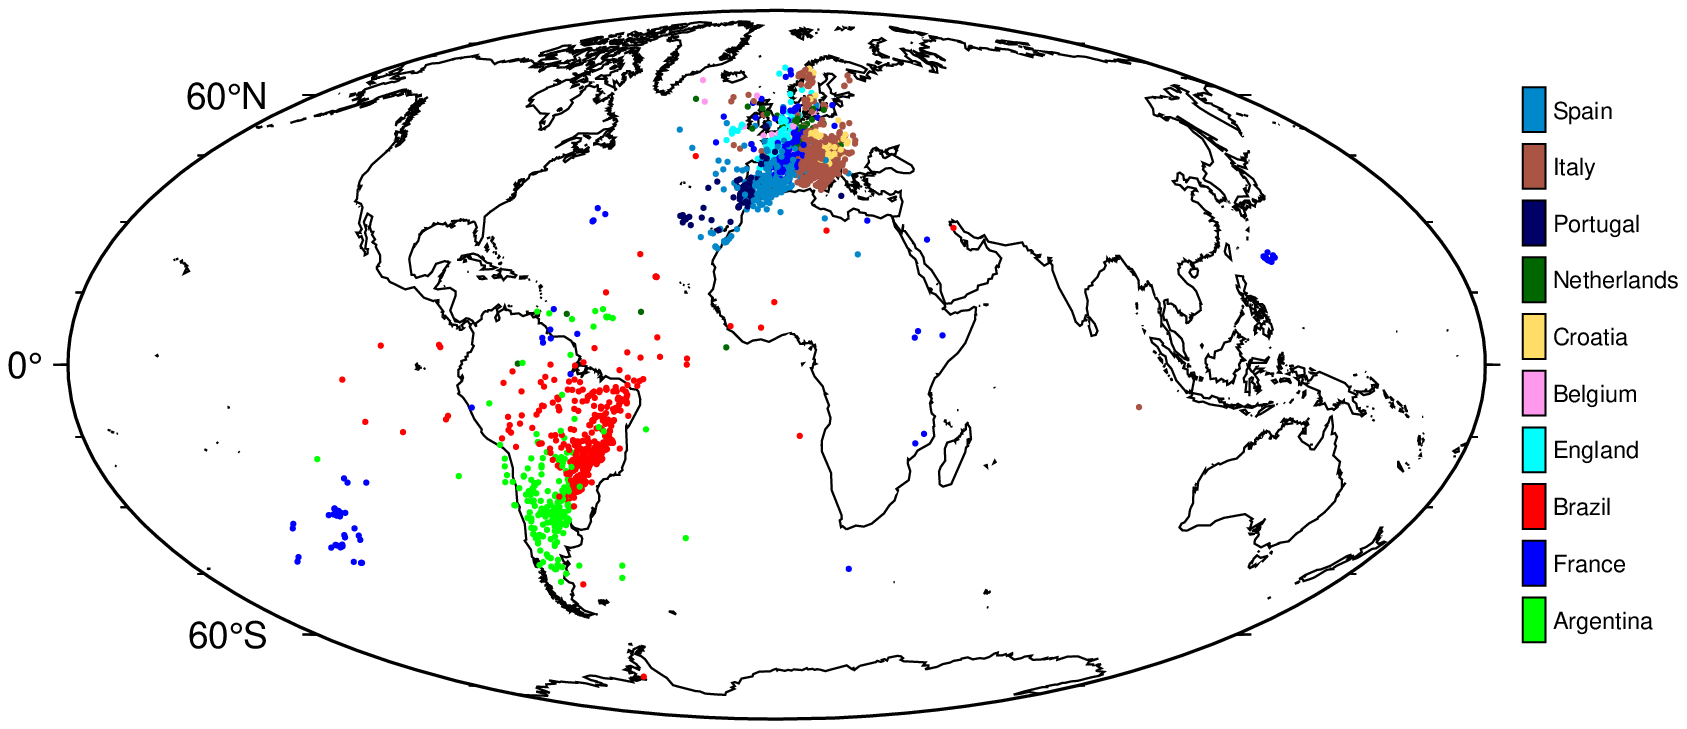
\includegraphics{results/figures/map.png}

}

\caption{\label{fig-map}Probe predictions for a random projection.}

\end{figure}

While this is admittedly a somewhat contrived example, it serves to
illustrate the point that if we randomly project a small number of
features that are highly correlated or predictive of the target into a
large enough space, we should expect to be able to recover meaningful
represenations of the target from the latent space. Similarly, Alain and
Bengio (2018) observe that even before training a convolutional neural
network on MNIST data, the layer-wise activations can already be used to
perform binary classification. In fact, it is well-known that random
projections can be used for prediction tasks (Dasgupta 2013).

\hypertarget{example-pca}{%
\subsection{Example: PCA}\label{example-pca}}

\hypertarget{example-autoencoder}{%
\subsection{Example: Autoencoder}\label{example-autoencoder}}

\hypertarget{example-llm}{%
\subsection{Example: LLM}\label{example-llm}}

\hypertarget{references}{%
\subsection*{References}\label{references}}
\addcontentsline{toc}{subsection}{References}

\hypertarget{refs}{}
\begin{CSLReferences}{1}{0}
\leavevmode\vadjust pre{\hypertarget{ref-alain2018understanding}{}}%
Alain, Guillaume, and Yoshua Bengio. 2018. {``Understanding Intermediate
Layers Using Linear Classifier Probes.''}
\url{https://arxiv.org/abs/1610.01644}.

\leavevmode\vadjust pre{\hypertarget{ref-dasgupta2013experiments}{}}%
Dasgupta, Sanjoy. 2013. {``Experiments with Random Projection.''}
\url{https://arxiv.org/abs/1301.3849}.

\leavevmode\vadjust pre{\hypertarget{ref-gurnee2023language}{}}%
Gurnee, Wes, and Max Tegmark. 2023. {``Language Models Represent Space
and Time.''} \url{https://arxiv.org/abs/2310.02207}.

\leavevmode\vadjust pre{\hypertarget{ref-touvron2023llama}{}}%
Touvron, Hugo, Thibaut Lavril, Gautier Izacard, Xavier Martinet,
Marie-Anne Lachaux, Timothée Lacroix, Baptiste Rozière, et al. 2023.
{``LLaMA: Open and Efficient Foundation Language Models.''}
\url{https://arxiv.org/abs/2302.13971}.

\end{CSLReferences}



\end{document}
